\documentclass[12pt,a4paper]{article}
\usepackage{ucebnice}

\title{Lineární funkce}
\author{Ondřej Škubala}
\date{\today}

\begin{document}

\maketitle
\newpage



\section{Lineární funkce}

\begin{quotebox}
{„Znalost přímky je klíčem k pochopení všech ostatních křivek.“}
{René Descartes, \textit{La Géométrie (1637)}}
\end{quotebox}

Lineární funkce patří k nejdůležitějším a zároveň nejjednodušším typům funkcí, se kterými se v matematice setkáváme.  
Jejich grafem je přímka, a právě proto tvoří přirozený most mezi algebrou a geometrií.  
Na příkladu lineárních funkcí si ukážeme, jak lze matematicky vyjádřit \textbf{rovnoměrné závislosti} – vztahy, při nichž se jedna veličina mění stále stejným způsobem, například závislost dráhy na čase při rovnoměrném pohybu, ceny na množství zboží nebo napětí na proudu.

Cílem této kapitoly je:
\begin{itemize}
    \item porozumět tomu, co znamená výraz \(y = ax + b\),
    \item vysvětlit význam koeficientů \(a\) a \(b\),
    \item naučit se číst a zakreslovat grafy lineárních funkcí,
    \item a umět podle zadaných informací určit rovnici přímky.
\end{itemize}

Dříve než přejdeme k příkladům, přesně si pojem \important{lineární funkce} definujeme.

\begin{definitionbox}
\important{Lineární funkce} je každá funkce na množině reálných čísel, tedy funkce, jejíž definiční obor je \(D(f) = \mathbb{R}\),  
a kterou lze vyjádřit předpisem
\[
f:\quad y = ax + b,
\]
kde \(a, b \in \mathbb{R}\) jsou \textbf{koeficienty lineární funkce}.  

\begin{itemize}
    \item \(a\) se nazývá \textbf{směrnice přímky} a určuje, jak rychle se hodnota \(y\) mění při změně \(x\);
    \item \(b\) je \textbf{posunutí (průsečík s osou \(y\))} a udává, jaká je funkční hodnota v bodě \(x=0\).
\end{itemize}
\end{definitionbox}

Proměnná \(x\) se nazývá \textbf{nezávisle proměnná} (argument funkce)  
a proměnná \(y\) je \textbf{závisle proměnná} (funkční hodnota).  
Každému číslu \(x\) z množiny reálných čísel přiřazuje funkce právě jednu hodnotu \(y\).  

% --- POPIS S ODKAZY NA GRAFY ---

Grafem lineární funkce je vždy \textbf{přímka}, jejíž tvar závisí na směrnici \(a\):

\begin{itemize}
    \item \textbf{Je-li \(a>0\), funkce je \hyperlink{rostouci}{rostoucí.}}  
    Hodnota \(y\) se zvyšuje se vzrůstajícím \(x\); graf má sklon směrem nahoru.

    \item \textbf{Je-li \(a<0\), funkce je \hyperlink{klesajici}{klesající.}}  
    Hodnota \(y\) se s rostoucím \(x\) zmenšuje; graf má sklon směrem dolů.

    \item \textbf{Je-li \(a=0\), funkce je \hyperlink{konstantni}{konstantní.}}  
    Všechny hodnoty \(y\) jsou stejné, graf je vodorovná přímka.
\end{itemize}


% --- GRAFY LINEÁRNÍCH FUNKCÍ ---
\begin{center}
\begin{minipage}[t]{0.32\textwidth}
    \vspace{0pt}
    \centering
    \hypertarget{rostouci}{}
    \begin{axisgraph}[
        xmin=-3, xmax=3,
        ymin=-3, ymax=3,
        width=\linewidth,
        height=5cm,
        axis lines=middle,
        grid=none,
        domain=-3:3,
        title={Rostoucí funkce}
    ]
        \addplot[thick, blue] {x + 1};
        \node at (rel axis cs:0.85,0.85) {\small $a>0$};
    \end{axisgraph}
\end{minipage}\hfill
\begin{minipage}[t]{0.32\textwidth}
    \vspace{0pt}
    \centering
    \hypertarget{klesajici}{}
    \begin{axisgraph}[
        xmin=-3, xmax=3,
        ymin=-3, ymax=3,
        width=\linewidth,
        height=5cm,
        axis lines=middle,
        grid=none,
        domain=-3:3,
        title={Klesající funkce}
    ]
        \addplot[thick, red] {-x + 1};
        \node at (rel axis cs:0.85,0.85) {\small $a<0$};
    \end{axisgraph}
\end{minipage}\hfill
\begin{minipage}[t]{0.32\textwidth}
    \vspace{0pt}
    \centering
    \hypertarget{konstantni}{}
    \begin{axisgraph}[
        xmin=-3, xmax=3,
        ymin=-3, ymax=3,
        width=\linewidth,
        height=5cm,
        axis lines=middle,
        grid=none,
        domain=-3:3,
        title={Konstantní funkce}
    ]
        \addplot[thick, black] {1};
        \node at (rel axis cs:0.85,0.85) {\small $a=0$};
    \end{axisgraph}
\end{minipage}
\end{center}

Na obrázcích výše vidíme, jak hodnota směrnice \(a\) ovlivňuje tvar grafu lineární funkce.  

Zápis \(y = ax + b\) tedy představuje nejen \textbf{funkční předpis},  
ale zároveň i \textbf{rovnici přímky} v souřadnicové rovině.  
Každý bod \([x; y]\) grafu splňuje tento vztah, a proto lze přecházet mezi algebraickým a geometrickým pohledem.  
Tím se ukazuje hluboké propojení mezi dvěma oblastmi matematiky – algebrou a geometrií. A tady toho propojení 
poznáme více v oboru analytické geometrie.


\begin{notebox}
\textbf{Důkaz monotonicity lineární funkce \(f(x)=ax+b\)}

\textbf{(i) Rostoucí pro \(a>0\).}  
Chceme ověřit, že pro všechna \(x_1,x_2\in\mathbb{R}\) platí
\[
x_1<x_2 \;\Rightarrow\; f(x_1)<f(x_2).
\]
Nechť \(x_1<x_2\). Protože \(a>0\), vynásobením kladným číslem se směr nerovnosti nemění, tedy
\[
a x_1 < a x_2.
\]
Přičteme-li na obou stranách číslo \(b\), dostaneme
\[
a x_1 + b < a x_2 + b,
\]
což je právě \(f(x_1) < f(x_2)\). Funkce je tedy \textbf{rostoucí}.

\medskip
\textbf{(ii) Klesající pro \(a<0\).}  
Opět nechť \(x_1<x_2\). Protože \(a<0\), vynásobením záporným číslem se směr nerovnosti obrátí:
\[
a x_1 > a x_2.
\]
Po přičtení \(b\) dostáváme
\[
a x_1 + b > a x_2 + b \;\;\Rightarrow\;\; f(x_1)>f(x_2),
\]
tedy funkce je \textbf{klesající}.

\medskip
\textbf{(iii) Konstantní pro \(a=0\).}  
Máme \(f(x)=0\cdot x + b = b\) pro všechna \(x\in\mathbb{R}\), tedy jde o \textbf{konstantní} funkci.  
Zároveň \(\forall x_1\neq x_2\) platí \(f(x_1)=f(x_2)=b\), takže funkce \textbf{není prostá}.

\medskip
\textbf{Důsledek.} Pro \(a\neq 0\) je \(f\) přísně monotónní (rostoucí/klesající), a proto i \textbf{prostá}.
\end{notebox}



\begin{examplebox}
\textbf{Směrnice přímky a její význam}

Ve funkci \(y = ax + b\) zvolme libovolné číslo \(x_1 \in \mathbb{R}\) a porovnejme hodnoty funkce v bodech \(x_1\) a \(x_1 + 1\):

\[
[a(x_1 + 1) + b] - (a x_1 + b) = a x_1 + a + b - a x_1 - b = a.
\]

Číslo \(a\) tedy udává, o kolik se funkční hodnota \(y\) změní, když se argument \(x\) zvětší o \(1\).  
Proto se \(a\) nazývá \textbf{směrnice přímky} — vyjadřuje „přírůstek výšky na jednotku šířky“.

\medskip
Zůstaneme-li u lineární funkce \(y = ax + b\) a označíme ji \(f\), pak pro libovolná dvě různá reálná čísla \(x_1, x_2\) platí:

\[
\begin{aligned}
f(x_2) - f(x_1) &= (a x_2 + b) - (a x_1 + b) \\[4pt]
&= a(x_2 - x_1).
\end{aligned}
\]

Odtud po úpravě dostaneme obecný vztah:
\[
\boxed{a = \frac{f(x_2) - f(x_1)}{x_2 - x_1}}.
\]

Tento vzorec říká, že směrnice \(a\) je \textbf{podíl změny funkčních hodnot ku změně argumentů}  
a má stejný význam jako „přírůstek na jednotku“ v přímé úměře.
\end{examplebox}

\begin{center}
\begin{axisgraph}[
    xmin=-2, xmax=5,
    ymin=-1, ymax=4,
    enlarge x limits=0.15,  % ← přidá 15 % šířky vlevo i vpravo
    enlarge y limits=0.1,   % ← přidá 10 % výšky nahoře i dole
    clip=false,
    axis lines=middle,
    grid=none,
    xtick={1},
    ytick={1},
    title={Význam směrnice $a$}
]
    % přímka
    \addplot[thick, blue] {0.5*x + 0.75};

    % body
    % \addplot[only marks, mark=*, red] coordinates {(1.5,2.5) (3,5.5)};
    % \node[below left, red] at (axis cs:1.5,2.5) {$[x_1; f(x_1)]$};
    % \node[above right, red] at (axis cs:3,5.5) {$[x_2; f(x_2)]$};

    % pomocné čáry
    \draw[very thick, black] (axis cs:1.5,1.5) -- (axis cs:3.5,1.5);
    \draw[very thick, black] (axis cs:3.5,1.5) -- (axis cs:3.5,2.5);

    \draw[dashed, gray!80!black] (axis cs:1.5,0) -- (axis cs:1.5,1.5);
    \draw[dashed, gray!80!black] (axis cs:3.5,0) -- (axis cs:3.5,1.5);

    \draw[dashed, gray!80!black] (axis cs:0,1.5) -- (axis cs:1.5,1.5);
    \draw[dashed, gray!80!black] (axis cs:0,2.5) -- (axis cs:3.5,2.5);

    % popisky Δx, Δy
    \node[below, black] at (axis cs:2.5,1.5) {$\Delta x$};
    \node[right, black] at (axis cs:3.5,2) {$\Delta y$};
    \node[below, gray!80!black] at (axis cs:1.5,0) {$x_1$};
    \node[below, gray!80!black] at (axis cs:3.5,0) {$x_2$};
    \node[left, gray!80!black] at (axis cs:0,1.5) {$f(x_1)$};
    \node[left, gray!80!black] at (axis cs:0,2.5) {$f(x_2)$};
\end{axisgraph}
\end{center}

\noindent
Na obrázku je znázorněno, že směrnice \(a\) odpovídá poměru \(\frac{\Delta y}{\Delta x}\),  
tedy „jak rychle stoupá (nebo klesá) funkce“.  
Proto je \(a>0\) rostoucí, \(a<0\) klesající a \(a=0\) konstantní.




\subsection{Způsoby, jak vytvořit graf lineární funkce}

Graf funkce lze znázornit několika různými způsoby.  
Každý z nich má své výhody – někdy je vhodnější přesný postup pomocí tabulky,  
jindy stačí využít tvar funkce a znalost jejích vlastností.

\begin{enumerate}[label=\arabic*.]
% --- 1. TABULKOVÁ METODA ---
\item \textbf{Pomocí tabulky hodnot}

Vybereme několik hodnot proměnné \(x\) (např. \(-3, -1, 0, 1, 3\)) a dosadíme je do funkčního předpisu \(y = ax + b\).  
Získané dvojice \([x; y]\) představují body grafu, které zakreslíme do souřadnicové roviny a propojíme přímkou.  
Tento způsob se označuje také jako \textbf{tabulková metoda}.

\begin{examplebox}
    \textbf{Příklad:}  
    Mějme funkci \(f(x) = 2x - 1\).

    \medskip
    Sestavíme tabulku hodnot:

    \[
    \begin{array}{c|ccccc}
    x & -2 & -1 & 0 & 1 & 2 \\ \hline
    y & -5 & -3 & -1 & 1 & 3
    \end{array}
    \]

    Body grafu jsou tedy \([-2;-5]\), \([-1;-3]\), \([0;-1]\), \([1;1]\), \([2;3]\).  


    \begin{center}
    \begin{minipage}{0.45\textwidth}
    \centering
    \begin{axisgraph}[
        grid=none,
        xmin=-3, xmax=3,
        ymin=-6, ymax=5,
        title={Nanesení bodů z tabulky},
        xlabel={$x$},
        ylabel={$y$},
    ]
        \addplot[only marks, mark=*] coordinates {
            (-2,-5) (-1,-3) (0,-1) (1,1) (2,3)
        };
    \end{axisgraph}
    \end{minipage}
    \hfill
    \begin{minipage}{0.45\textwidth}
    \centering
    \begin{axisgraph}[
        grid=none,
        xmin=-3, xmax=3,
        ymin=-6, ymax=5,
        title={Funkce $f(x)=2x-1$},
        xlabel={$x$},
        ylabel={$y$},
    ]
        % body
        \addplot[only marks, mark=*] coordinates {
            (-2,-5) (-1,-3) (0,-1) (1,1) (2,3)
        };
        % přímka
        \addplot[thick, blue] {2*x - 1};
    \end{axisgraph}
    \end{minipage}
    \end{center}
\end{examplebox}


Na prvním obrázku jsou pouze body vypočtené z tabulky hodnot.  
Na druhém obrázku je těmito body proložena přímka, která znázorňuje průběh funkce \(f(x)=2x-1\).  
Tím jsme vytvořili graf lineární funkce pomocí tabulkové metody.


\medskip

% --- 2. SMĚRNICE A POSUN ---
\item \textbf{Pomocí znalosti směrnice a posunu}

Pokud známe koeficienty \(a\) a \(b\), můžeme graf nakreslit přímo:  
\begin{itemize}
    \item \(b\) určuje, kde přímka protne osu \(y\),  
    \item \(a\) určuje její sklon – o kolik se \(y\) změní, když se \(x\) zvětší o 1.
\end{itemize}

\begin{examplebox}
\textbf{Příklad:}  
Nakreslete graf funkce \(f(x) = \tfrac{1}{2}x + 2\).

\medskip
Přímka protíná osu \(y\) v bodě \([0;2]\) (protože \(b=2\)).  
Směrnice \(a=\tfrac{1}{2}\) znamená, že když \(x\) zvětšíme o 1, hodnota \(y\) se zvětší o \(\tfrac{1}{2}\).  
Z bodu \([0;2]\) tedy „postoupíme“ o 1 jednotku doprava a o \(\tfrac{1}{2}\) nahoru, čímž získáme druhý bod \([1;2{,}5]\).  
Přímku jimi propojíme – a graf je hotov.


\begin{center}
\begin{minipage}{0.45\textwidth}
\centering
\begin{axisgraph}[
    grid=none,
    xmin=-3, xmax=4,
    ymin=-1, ymax=4,
    title={Určení bodů podle $a$ a $b$},
    xlabel={$x$},
    ylabel={$y$},
    axis lines=middle,
    width=\linewidth,
    height=6cm
]
    % body
    \addplot[only marks, mark=*, blue] coordinates {(0,2) (1,2.5)};
    % pomocné čáry
    \draw[dashed, gray] (axis cs:0,2) -- (axis cs:1,2);
    \draw[dashed, gray] (axis cs:1,2) -- (axis cs:1,2.5);
    % popisky
    \node[above left, blue] at (axis cs:0,2) {$[0;2]$};
    \node[right, blue] at (axis cs:1,2.5) {$[1;2{,}5]$};
\end{axisgraph}
\end{minipage}
\hfill
\begin{minipage}{0.45\textwidth}
\centering
\begin{axisgraph}[
    grid=none,
    xmin=-3, xmax=4,
    ymin=-1, ymax=4,
    title={Graf funkce $f(x)=\tfrac{1}{2}x+2$},
    xlabel={$x$},
    ylabel={$y$},
    axis lines=middle,
    width=\linewidth,
    height=6cm,
    domain=-3:4,
    samples=2
]
    % přímka
    \addplot[thick, blue] {0.5*x + 2};
    % body
    \addplot[only marks, mark=*, red] coordinates {(0,2) (1,2.5)};
\end{axisgraph}
\end{minipage}
\end{center}
\end{examplebox}

Na levém obrázku jsou vyznačeny dva body zjištěné podle směrnice \(a\) a posunu \(b\).  
Na pravém obrázku vidíme výslednou přímku, která těmito body prochází.  
Tento postup je rychlý a přehledný – zejména pokud známe rovnice více lineárních funkcí a chceme je navzájem porovnat.

\medskip

% --- 4. TRANSFORMACE ---
\item \textbf{Pomocí transformací známé přímky}

Vycházíme ze základní funkce \(f(x) = x\).  
Násobení koeficientem \(a\) přímku nakloní (změní sklon),  
a přičtení čísla \(b\) ji posune nahoru nebo dolů.

\begin{examplebox}
\textbf{Příklad:}  
Začněme se základní přímkou \(\textcolor{blue}{f(x)=x}\).  
Pokud ji vynásobíme číslem 2, získáme \(\textcolor{pastelorange}{f(x)=2x}\) – přímka je strmější.  
Pokud pak přičteme \(b=-3\), dostaneme \(\textcolor{green!50!black}{f(x)=2x-3}\) –  
přímku se stejným sklonem, ale posunutou dolů o 3 jednotky.


Naopak přidání kladného \(b\) posune přímku nahoru.


\begin{center}
    \begin{minipage}[t]{0.32\textwidth}
        \centering
        \begin{axisgraph}[
            grid=none,
            xmin=-3, xmax=3,
            ymin=-4, ymax=4,
            title={$f(x)=x$},
            axis lines=middle,
            width=\linewidth,
            height=5.5cm,
            domain=-3:3,
            samples=2
        ]
            \addplot[thick, blue] {x};
        \end{axisgraph}
    \end{minipage}\hfill
    \begin{minipage}[t]{0.32\textwidth}
        \centering
        \begin{axisgraph}[
            grid=none,
            xmin=-3, xmax=3,
            ymin=-4, ymax=4,
            title={$f(x)=2x$},
            axis lines=middle,
            width=\linewidth,
            height=5.5cm,
            domain=-3:3,
            samples=2
        ]
            \addplot[thick, pastelorange] {2*x};
        \end{axisgraph}
    \end{minipage}\hfill
    \begin{minipage}[t]{0.32\textwidth}
        \centering
        \begin{axisgraph}[
            grid=none,
            xmin=-3, xmax=3,
            ymin=-4, ymax=4,
            title={$f(x)=2x-3$},
            axis lines=middle,
            width=\linewidth,
            height=5.5cm,
            domain=-3:3,
            samples=2
        ]
            \addplot[thick, green!50!black] {2*x - 3};
        \end{axisgraph}
    \end{minipage}
\end{center}
\end{examplebox}

\end{enumerate}


\subsection{Průsečíky grafu s osami}

Každý graf lineární funkce \(f(x)=ax+b;\; a \neq 0\) protíná obě osy souřadnic (právě pokud není rovnoběžný s některou z nich).

\begin{itemize}
    \item \textbf{Průsečík s osou $y$} získáme dosazením \(x=0\).  
    \item \textbf{Průsečík s osou $x$} určíme tak, že položíme \(f(x)=0\) a vypočítáme \(x\).
\end{itemize}

\bigskip
\begin{examplebox}
Najděte průsečíky grafu funkce \(f(x) = 2x - 4\) s osami souřadnic.

\bigskip
\textbf{Průsečík s osou $y$:}

dosadíme $x = 0$
\[
\begin{aligned}
    y &= 2\cdot 0 - 4,\\[4pt]
    y &= -4 \quad \text{tedy bod } [0;-4].
\end{aligned}
\]

\bigskip
\textbf{Průsečík s osou $x$:}

řešíme rovnici $y = 2x - 4$ pro $y=0$
\[
\begin{aligned}
    y &= 2x - 4,\\[4pt]
    0 &= 2x - 4 ,\\[4pt]
    x &= 2, \quad \text{tedy bod} [2;0].    
\end{aligned}
\]

\bigskip
\textbf{Graficky:}


\begin{center}
    \begin{axisgraph}[
        grid=none,
        xmin=-1, xmax=3,
        ymin=-5, ymax=2,
        title={Průsečíky s osami: $f(x)=2x-4$},
        xlabel={$x$},
        ylabel={$y$},
        axis lines=middle,
        width=9cm,
        height=6cm,
        domain=-0.5:2.5,
        samples=2
    ]
        \addplot[thick, blue] {2*x - 4};
        \addplot[only marks, mark=*, red] coordinates {(0,-4) (2,0)};
    \end{axisgraph}
\end{center}
\end{examplebox}

Průsečík s osou \(y\) určuje posunutí přímky (koeficient \(b\)),  
zatímco průsečík s osou \(x\) ukazuje, kdy má funkce nulovou hodnotu \(f(x)=0\).


\section{Parametrické zavedení lineárních funkcí}

V matematice se často nesetkáváme pouze s jednou konkrétní funkcí,  
ale s celou \textbf{množinou funkcí}, které mají podobný tvar,  
liší se však hodnotami některých číselných koeficientů.  
Tato čísla nazýváme \important{parametry} a způsob, jakým funkci zapisujeme pomocí těchto parametrů,  
se nazývá \important{parametrické zavedení funkce}.

\begin{definitionbox}
Řekneme, že funkce \(f(x)\) je \textbf{parametricky zavedena},  
jestliže její předpis obsahuje jedno nebo více čísel (parametrů),  
jejichž konkrétní volbou získáme různé funkce téhož typu.

Například funkce
\[
f(x) = a x + b
\]
je parametricky zavedena pomocí parametrů \(a\) a \(b\).
\end{definitionbox}

Volbou konkrétních hodnot těchto parametrů tedy získáváme různé členy jedné \textbf{rodiny lineárních funkcí}.

\begin{itemize}
    \item Parametr \(a\) určuje \textbf{směrnici} přímky (její sklon).  
    \item Parametr \(b\) určuje \textbf{posunutí} přímky na ose \(y\).
\end{itemize}

\medskip
\textbf{Jinými slovy:} když necháme parametry \(a\) a \(b\) volně měnit,  
můžeme sledovat, jak se mění tvar celé skupiny lineárních funkcí.

\newpage
\begin{examplebox}
\textbf{Změna směrnice \(a\):}  

Mějme rodinu funkcí 
\[
f(x):\quad y = a x + 1, \qquad a \in \{-2; -1; 0; 1; 2\}.
\]
Zde je parametr \(a\) proměnný, zatímco \(b = 1\) je pevné.

\[
\begin{array}{c|c}
a & \text{Předpis funkce} \\ \hline
\textcolor{blue}{-3}  & f(x) = -3x + 1 \\
\textcolor{black!50}{0}  & f(x) = 1 \\
\textcolor{orange}{1}  & f(x) = x + 1 \\
\textcolor{green!50!black}{0}  & f(x) = 2x + 1
\end{array}
\]

\begin{center}
\begin{axisgraph}[
    grid=none,
    xmin=-3, xmax=3,
    ymin=-3, ymax=5,
    title={Různé hodnoty $a$ při $b=1$},
    axis lines=middle,
    width=9cm,
    height=6cm,
    domain=-3:3,
    samples=2
]
    \addplot[thick, blue] {2*x + 1};
    \addplot[thick, black!50] {1};
    \addplot[thick, orange] {-x + 1};
    \addplot[thick, green!50!black] {-3*x + 1};
\end{axisgraph}
\end{center}

Z grafu vidíme, že při růstu parametru \(a\) se přímka stává strmější,  
zatímco při záporných hodnotách \(a\) se její směr obrací.  
Při \(a = 0\) dostáváme konstantní funkci \(f(x) = 1\).
\end{examplebox}




\begin{examplebox}
\textbf{Změna posunu \(b\):}  

Mějme rodinu funkcí 
\[
f(x):\quad y = 2x + b, \qquad b \in \{-3; 0; 2; 4\}.
\]
Zde je parametr \(b\) proměnný, zatímco \(a = 2\) je pevné.

\[
\begin{array}{c|c}
b & \text{Předpis funkce} \\ \hline
\textcolor{green!50!black}{-3} & f(x) = 2x - 3 \\
\textcolor{black!70}{0} & f(x) = 2x \\
\textcolor{red}{2} & f(x) = 2x + 2 \\
\textcolor{blue}{4} & f(x) = 2x + 4
\end{array}
\]


\begin{center}
\begin{axisgraph}[
    grid=none,
    xmin=-3, xmax=3,
    ymin=-4, ymax=6,
    title={Různé hodnoty $b$ při $a=2$},
    axis lines=middle,
    width=9cm,
    height=6cm,
    domain=-3:3,
    samples=2
]
    \addplot[thick, blue] {2*x + 4};
    \addplot[thick, red] {2*x + 2};
    \addplot[thick, black!70] {2*x};
    \addplot[thick, green!50!black] {2*x - 3};
\end{axisgraph}
\end{center}

Všechny přímky mají stejnou směrnici \(a = 2\), a tedy i stejný sklon.  
Liší se však hodnotou parametru \(b\), který způsobuje posunutí přímky  
nahoru (pro \(b>0\)) nebo dolů (pro \(b<0\)).  
Tímto způsobem získáváme \textbf{rodinu rovnoběžných přímek}.
Zároveň si můžeme ještě jednou povšimnout, že skutečně hodnoty parametru $b$ 
souvisí s hodnotou průsečíku lienární funkce a osy $y$ grafu.
\end{examplebox}


\newpage
\begin{examplebox}
\textbf{Příklad 3 – spojitá změna parametru \(b\):}  

Uvažujme rodinu lineárních funkcí
\[
f(x) = 2x + b, \qquad b \in \langle -1; 1 \rangle.
\]

Parametr \(a = 2\) je pevný, určuje tedy sklon všech přímek.  
Parametr \(b\) se mění v intervalu od \(-1\) do \(1\), což znamená,  
že přímky se posouvají plynule nahoru a dolů, aniž by se změnil jejich sklon.

\medskip
Z geometrického hlediska tedy dostáváme \textbf{nekonečně mnoho rovnoběžných přímek},  
které se liší pouze polohou.

\begin{center}
\begin{axisgraph}[
    grid=none,
    xmin=-3, xmax=3,
    ymin=-3, ymax=5,
    title={Rodina přímek $f(x)=2x+b$, kde $b\in\langle -1;1\rangle$},
    axis lines=middle,
    width=10cm,
    height=6cm,
    domain=-3:3,
    samples=2
]
    % krajní přímky (tlusté, tmavě modré)
    \addplot[ultra thick, blue!80!black] {2*x - 1};
    \addplot[ultra thick, blue!80!black] {2*x + 1};

    % mezilehlé přímky (světlejší, čárkované)
    \addplot[thick, dashed, blue!40] {2*x - 0.75};
    \addplot[thick, dashed, blue!40] {2*x - 0.5};
    \addplot[thick, dashed, blue!40] {2*x - 0.25};
    \addplot[thick, dashed, blue!40] {2*x + 0};
    \addplot[thick, dashed, blue!40] {2*x + 0.25};
    \addplot[thick, dashed, blue!40] {2*x + 0.5};
    \addplot[thick, dashed, blue!40] {2*x + 0.75};

\end{axisgraph}
\end{center}

\noindent
Na grafu jsou zvýrazněny dvě krajní přímky odpovídající hodnotám \(b=-1\) a \(b=1\).  
Všechny ostatní přímky mezi nimi (čárkované) představují různé hodnoty \(b\) z intervalu \(\langle -1;1\rangle\).  
Protože mají všechny stejnou směrnici \(a=2\), jsou rovnoběžné.  
Tento způsob zápisu vyjadřuje tzv. \textbf{parametrické zavedení funkce podle $b$}.
\end{examplebox}

\begin{notebox}
\textbf{Poznámka – „Lineární“ neznamená vždy „přímka“}

Na střední škole označujeme jako \textbf{lineární funkce} všechny funkce tvaru
\[
f(x) = ax + b,
\]
jejichž grafem je přímka.  
Z formálního hlediska se ale tyto funkce správně nazývají \textbf{afinní funkce}  
(od slova \textit{affinis} – „příbuzný, podobný“).  

Skutečně \emph{lineární} v přísném matematickém smyslu je jen ta funkce, která splňuje dvě vlastnosti:
\[
f(x+y) = f(x) + f(y), \qquad f(kx) = k\,f(x)
\]
pro všechna reálná čísla \(x, y\) a \(k\).  
Taková funkce má vždy tvar
\[
f(x) = ax,
\]
tedy přímku, která prochází počátkem souřadnic \([0;0]\).  
Přidáním členu \(b\) (tj. posunutím přímky) dostáváme již funkci \textbf{afinní}, nikoliv striktně lineární.

\medskip
Z hlediska středoškolské matematiky je tento rozdíl obvykle zanedbatelný,  
ale později – v \textbf{lineární algebře} – bude mít zásadní význam.
\end{notebox}






% --- PŘECHOD K LINEÁRNÍ GEOMETRII ---
\section{Návaznosti na budoucí látky}

\begin{notebox}
\textbf{Poznámka – „Lineární“ neznamená vždy „přímka“}

Ve školní matematice označujeme jako \textbf{lineární funkce} všechny funkce tvaru
\[
f(x) = ax + b,
\]
jejichž grafem je přímka.  
Z přesnějšího matematického hlediska se však tyto funkce nazývají \textbf{afinní funkce},  
protože zahrnují nejen „sklon“ (určený parametrem \(a\)), ale i „posunutí“ (parametr \(b\)).  

Skutečně \emph{lineární} v úzkém smyslu jsou pouze ty funkce, jejichž graf prochází počátkem souřadnic,  
tedy \(f(x) = ax\).  

Přidání posunutí o \(b\) už mění funkci z „čistě lineární“ na „afinní“,  
což si více uvědomíme při studiu \textbf{lineární geometrie},  
kde budeme zkoumat obecné přímky, jejich rovnoběžnost, kolmost i vzájemnou polohu.
\begin{center}
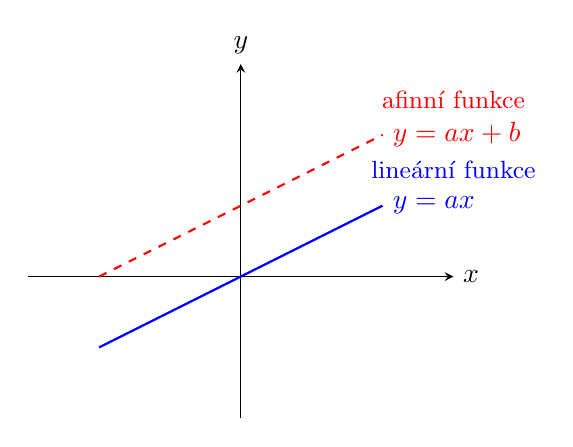
\begin{tikzpicture}[scale=0.9,>=stealth]
    % souřadnicové osy
    \draw[->] (-3,0) -- (3,0) node[right] {$x$};
    \draw[->] (0,-2) -- (0,3) node[above] {$y$};

    % přímky
    \draw[thick, blue] (-2,-1) -- (2,1) node[right, blue] {$y=ax$};
    \draw[thick, red, dashed] (-2,0) -- (2,2) node[right, red] {$y=ax+b$};

    % popisky
    \node[blue] at (3,1.5) {\small lineární funkce};
    \node[red] at (3.0,2.5) {\small afinní funkce};
\end{tikzpicture}
\end{center}
\end{notebox}

\begin{notebox}
\textbf{Co si zapamatovat}
\begin{itemize}
    \item Lineární funkce \(f(x)=ax+b\) je základní příklad přímé závislosti mezi veličinami.
    \item Koeficient \(a\) určuje směrnici přímky (sklon), \(b\) určuje posunutí (průsečík s osou \(y\)).
    \item Pokud \(a=0\), dostáváme konstantní funkci. Pokud \(b=0\), graf prochází počátkem.
    \item Funkce \(f(x)=ax\) je „lineární“ v úzkém matematickém smyslu,  
          funkce \(f(x)=ax+b\) je „afinní“ – posunutá přímka.
    \item Studium těchto vlastností je základem pro \textbf{analytickou geometrii},  
          která zkoumá polohy přímek, rovin a jejich vzájemné vztahy.
\end{itemize}
\end{notebox}








% -----------------------------------------------------------------
% ---------------------- P Ř Í K L A D Y — LINEÁRNÍ FUNKCE --------
% -----------------------------------------------------------------

\exercisepart
\setcounter{section}{1} % případně uprav dle předchozího číslování


% =========================
% ÚLOHA 1
% =========================
\begin{exercise}[Parametry $a,b$ v předpisu $y=ax+b$]
    Určete hodnoty parametrů $a,b$ následujících funkcí:
    \begin{tasks}(2)
        \task $y=10{,}8x+500$
        \task $y=10{,}8x$
        \task $y=3{,}6x+500$
        \task $y=-3{,}6x+500$
        \task $y=650+10{,}8x$
        \task $y=2\cdot(120x+40)+120$
    \end{tasks}
\end{exercise}


% =========================
% ÚLOHA 2
% =========================
\begin{exercise}[Rychlé náčrty grafů lineárních funkcí]
    Načrtněte grafy uvedených funkcí:
    \begin{tasks}(3)
        \task $y=1{,}5$
        \task $y=3$
        \task $y=-\pi$
        \task $y=2x$
        \task $y=3x$
        \task $y=-0{,}5x$
        \task $y=x+2$
        \task $y=-2x+4$
        \task $y=0{,}5x-1$
        \task $y=x-3$
        \task $y=\dfrac{3}{2}x-1$
        \task $y=-\dfrac{3}{2}x+1$
    \end{tasks}
\end{exercise}


% =========================
% ÚLOHA 3
% =========================
\begin{exercise}[Proč svislá přímka není grafem funkce]
    Zdůvodněte, že přímka rovnoběžná s osou $y$ (tj. $x=c$) nemůže být grafem žádné funkce vyjadřující závislost $y$ na $x$.
\end{exercise}


% =========================
% ÚLOHA 4
% =========================
\begin{exercise}[Předpis lineární funkce z hodnot I]
    Pro lineární funkci $h$ platí $h(3)=-5$ a $h(-1)=4$. Zapište ji předpisem $y=ax+b$ a sestrojte její graf.
\end{exercise}


% =========================
% ÚLOHA 5
% =========================
\begin{exercise}[Předpis lineární funkce z hodnot II]
    Zapište rovnici lineární funkce $f$, víte-li, že platí $f(0)=1$ a $f(2)=5$; poté načrtněte její graf.
\end{exercise}


% =========================
% ÚLOHA 6
% =========================
\begin{exercise}[Předpis lineární funkce z hodnot III]
    Zapište rovnici lineární funkce $g$, víte-li, že platí $g(x+1)-g(x)=2$ a $g(0)=3$; poté načrtněte její graf.
\end{exercise}


% =========================
% ÚLOHA 7
% =========================
\begin{exercise}[Rovnice lineární funkce z daných bodů I]
    Lineární funkce $f$ prochází body $[1;1]$ a $[3;-2]$.  
    Určete její předpis a sestrojte graf funkce:
    \begin{tasks}(1)
        \task $* $ pomocí soustavy souřadnic,
        \task pomocí významu konstant $a,b$ v předpisu $y=ax+b$.
    \end{tasks}
\end{exercise}


% =========================
% ÚLOHA 8
% =========================
\begin{exercise}[Rovnice lineární funkce z daných bodů II]
    Lineární funkce $g$ prochází body $[1;2]$ a $[3;-4]$.  
    Určete její předpis a sestrojte graf funkce.
\end{exercise}


% =========================
% ÚLOHA 9
% =========================
\begin{exercise}[Rovnice lineární funkce z daných bodů III]
    Lineární funkce $h$ prochází body $[-4;-1]$ a $[1;1]$.  
    Určete její předpis a sestrojte graf funkce.
\end{exercise}


% =========================
% ÚLOHA 10
% =========================
\begin{exercise}[Graf a čtení nerovností z grafu]
    Sestrojte graf funkce $f\colon y=-x+2{,}5$. Z grafu určete všechna $x\in\mathbb{R}$, pro která platí:
    \begin{tasks}(3)
        \task $f(x)=0$
        \task $f(x)\le 0$
        \task $f(x)>3$
        \task $f(x)\le -1$
        \task $-3\le f(x)\le 2$
        \task $-7{,}5<f(x)<4{,}5$
    \end{tasks}
\end{exercise}


% =========================
% ÚLOHA 11
% =========================
\begin{exercise}[Porovnání dvou přímek v jedné soustavě]
    Sestrojte v téže soustavě souřadnic $Oxy$ grafy funkcí
    \[
        f_{1}\colon y=x+1,\qquad f_{2}\colon y=-0{,}5x+4.
    \]
    Určete všechna $x\in\mathbb{R}$, pro která platí:
    \begin{tasks}(2)
        \task $x+1=-0{,}5x+4$
        \task $x+1\le -0{,}5x+4$
        \task $x+1< -0{,}5x+4$
        \task $x+1\ge -0{,}5x+4$
        \task $x+1> -0{,}5x+4$
    \end{tasks}
\end{exercise}


% =========================
% ÚLOHA 12
% =========================
\begin{exercise}[Odečítání hodnot z grafu dvou funkcí]
    Sestrojte v téže soustavě souřadnic $Oxy$ grafy funkcí
    \[
        g_{1}\colon y=0{,}5x-2,\qquad g_{2}\colon y=-x-1.
    \]
    Z obrázku určete, které z následujících výroků jsou pravdivé:
    \begin{tasks}(2)
        \task $g_{1}(0)>g_{2}(0)$
        \task $g_{1}(4)\ge g_{2}(4)$
        \task $g_{1}(-2)<g_{2}(-2)$
        \task $g_{1}(3)\le g_{2}(3)$
    \end{tasks}
\end{exercise}


% =========================
% ÚLOHA 13
% =========================
\begin{exercise}[Příklady rostoucích a klesajících lineárních funkcí]
    Uvádějte příklady lineárních funkcí, které jsou:
    \begin{tasks}(2)
        \task rostoucí,
        \task klesající.
    \end{tasks}
\end{exercise}


% =========================
% ÚLOHA 14
% =========================
\begin{exercise}[Rychlý náčrt z parametrů $a,b$]
    Načrtněte graf lineární funkce $y=ax+b$ pro:
    \begin{tasks}(2)
        \task $a=0{,}5,\; b=-1$
        \task $a=-2,\; b=0{,}8$
    \end{tasks}
\end{exercise}


% =========================
% ÚLOHA 15
% =========================
\begin{exercise}[Směrnice z dané hodnoty a konstanty]
    Pro lineární funkci $y=ax+b$ platí $b=-3$ a $f(2)=5$. Určete směrnici $a$, rozhodněte, zda je funkce rostoucí, či klesající, a sestrojte graf.
\end{exercise}


\newpage
% =========================
% ÚLOHA 16
% =========================
\begin{exercise}[Předpis z hodnot ve dvou bodech]
    O lineární funkci $f$ je známo, že $f(1)=1{,}5$ a $f(-2)=-9$. Rozhodněte, zda je $f$ rostoucí, nebo klesající, a vyjádřete ji předpisem $y=ax+b$.
\end{exercise}


% =========================
% ÚLOHA 17
% =========================
\begin{exercise}[Rodina přímek se stejnou směrnicí]
    Načrtněte v téže soustavě souřadnic $Oxy$ grafy funkcí $y=0{,}7x+b$ pro $b\in\{-3;\,-1{,}5;\,0;\,1{,}5;\,2\}$.
\end{exercise}


% =========================
% ÚLOHA 18
% =========================
\begin{exercise}[Rodina přímek se stejným průsečíkem s osou $y$]
    Načrtněte v téže soustavě souřadnic $Oxy$ grafy funkcí $y=ax+3$ pro $a\in\{0;\,-3;\,-4;\,1{,}4;\,5\}$.
\end{exercise}


% =========================
% ÚLOHA 19
% =========================
\begin{exercise}[Porovnání dvou lineárních funkcí v jedné soustavě]
    Sestrojte v téže soustavě souřadnic $Oxy$ grafy funkcí
    \[
        k_1:\; y=3x-1,\qquad k_2:\; y=x+4.
    \]
    \begin{tasks}(1)
        \task Určete všechna $x\in\mathbb{R}$, pro která platí: $k_1(x)\ge 0$;\; $k_1(x)<-1$;\; $k_2(x)<0$;\; $k_2(x)\ge 4$.
        \task Určete všechna $x\in\mathbb{R}$, pro která platí: $k_1(x)\ge k_2(x)$;\; $k_1(x)<k_2(x)$.
        \task Určete z obrázku řešení soustavy rovnic $y=3x-1$,\; $y=x+4$ s neznámými $x,y\in\mathbb{R}$.
    \end{tasks}
\end{exercise}


% =========================
% ÚLOHA 20
% =========================
\begin{exercise}[Po částech lineární funkce]
    Nakreslete graf funkce $f$, která je po částech lineární a pro kterou platí: 
    $D(f)=\langle -5,\infty)$, $f(-5)=0$; 
    pro $x=0$ má $f$ maximum $5$; 
    na $\langle -5,0\rangle$ je $f$ rostoucí, na $\langle 0,4\rangle$ klesající a $f(4)=-5$; 
    na $\langle 4,\infty)$ je $f$ konstantní.  
    Zapište $f$ jako sjednocení lineárních funkcí.
\end{exercise}


% =========================
% ÚLOHA 21
% =========================
\begin{exercise}[Náčrty grafů po částech]
    Načrtněte grafy funkcí $f_1$ a $f_2$:
    \[
    f_1(x)=
    \begin{cases}
        x, & \text{pokud } x\ge 0,\\
        -x, & \text{pokud } x<0,
    \end{cases}
    \qquad
    f_2(x)=
    \begin{cases}
        1, & \text{pokud } x\ge 2,\\
        2x+1, & \text{pokud } x<2.
    \end{cases}
    \]
\end{exercise}


% =========================
% ÚLOHA 22
% =========================
\begin{exercise}[Souměrnost grafu lineární funkce]
    Je dána funkce $g\colon y=-2x+3$.  
    Určete funkční předpis lineární funkce $f$ tak, aby graf funkce $f$ byl souměrný s grafem funkce $g$ podle:
    \begin{tasks}(2)
        \task osy $x$,
        \task osy $y$,
        \task počátku soustavy souřadnic,
        \task $* $ přímky $y=x$.
    \end{tasks}
\end{exercise}


\newpage
\setcounter{section}{2}
% =========================
% ÚLOHA 23
% =========================
\begin{exercise}[Orlík — plnění nádrže]
Celková kapacita přehradní nádrže Orlík je \(3{,}780\,000\,000~\mathrm{m^3}\). Na začátku povodní bylo v nádrži \(3{,}500\,000\,000~\mathrm{m^3}\). Každou sekundu přiteče \(34\,000~\mathrm{m^3\,s^{-1}}\) a odtéká \(1\,000~\mathrm{m^3\,s^{-1}}\).
\begin{tasks}
\task Spočítejte, kolik vody přibude za \(1\,\mathrm{s}\), \(1\,\mathrm{min}\) a \(1\,\mathrm{h}\).
\task Určete, kolik vody bude v nádrži po \(1\,\mathrm{h}\), \(2\,\mathrm{h}\), \(5\,\mathrm{h}\), \(10\,\mathrm{h}\) a \(1\,\mathrm{dnu}\).
\task Najděte funkci \(V(t)\), která udává množství vody (v milionech \(\mathrm{m^3}\)) v závislosti na čase \(t\) (v hodinách), určete její definiční obor a obor hodnot a narýsujte graf.
\task Určete, za jak dlouho bude nádrž zcela plná.
\end{tasks}
\end{exercise}

% =========================
% ÚLOHA 24
% =========================
\begin{exercise}[Orlík — varianty plnění/čerpaní]
Vyřešte předchozí úlohu pro tyto pozměněné situace (vždy uveďte předpis \(V(t)\) v milionech \(\mathrm{m^3}\), \(t\) v hodinách, a načrtněte graf):
\begin{tasks}
\task na začátku je nádrž zcela prázdná,
\task přítok je \(2\,000~\mathrm{m^3\,s^{-1}}\) a odtok \(1\,000~\mathrm{m^3\,s^{-1}}\),
\task přítok je \(1\,000~\mathrm{m^3\,s^{-1}}\) a odtok \(2\,000~\mathrm{m^3\,s^{-1}}\),
\task na začátku bylo \(3{,}650\,000\,000~\mathrm{m^3}\).
\end{tasks}
Nakreslete všechny čtyři grafy do jedné soustavy.
\end{exercise}

% =========================
% ÚLOHA 25
% =========================
\begin{exercise}[Dvě cenové strategie — kdy se vyplatí internet]
Petr kupuje oblíbenou sladkost. V místním obchodě stojí \(39{,}90~\mathrm{Kč}\) za kus, na internetu \(35~\mathrm{Kč}\) za kus a poštovné \(70~\mathrm{Kč}\).
\begin{tasks}
\task Sestavte funkce celkové ceny \(C_\mathrm{obch}(n)\) a \(C_\mathrm{net}(n)\) v závislosti na počtu kusů \(n\in\mathbb{N}\).
\task Určete, pro která \(n\) je výhodnější nákup přes internet a pro která v obchodě.
\task Znázorněte obě závislosti v jednom grafu (osa \(x\): počet kusů, osa \(y\): cena v Kč).
\end{tasks}
\end{exercise}

% =========================
% ÚLOHA 26
% =========================
\begin{exercise}[Rybník — odtok se stálým přítokem]
V rybníce je \(150\,000~\mathrm{m^3}\) vody. Po otevření stavidel odtéká \(10~\mathrm{m^3\,s^{-1}}\), stálý přítok je \(3~\mathrm{m^3\,s^{-1}}\).
\begin{tasks}
\task Určete funkci \(V(t)\) (množství vody v \(\mathrm{m^3}\)) v závislosti na čase \(t\) (v sekundách) od otevření stavidel.
\task Za jak dlouho bude rybník prázdný? (Je-li prázdnění možné.) Znázorněte graf.
\end{tasks}
\end{exercise}

% =========================
% ÚLOHA 27
% =========================
\begin{exercise}[SŠ vs. VŠ — celkové výdělky v čase]
V roce 2024 byl odhad průměrné čisté mzdy: středoškolák s maturitou \(36\,000~\mathrm{Kč}\) za měsíc, vysokoškolák \(47\,000~\mathrm{Kč}\) za měsíc. Vysokoškolák však 5 let studuje (0 příjem), zatímco středoškolák ihned pracuje. Roční částky zaokrouhlujte na tisíce.
\begin{tasks}
\task Sestavte funkce \(S(t)\) a \(V(t)\) (v tisících Kč) udávající celkově vydělanou částku v závislosti na počtu let \(t\) od maturity.
\task Po kolika letech od maturity bude mít průměrný vysokoškolák více než středoškolák?
\task Pokud oba odejdou do důchodu v 65 letech a maturovali v 19, určete rozdíl jejich celoživotních příjmů.
\end{tasks}
\end{exercise}

% =========================
% ÚLOHA 28
% =========================
\begin{exercise}[Interpretace parametru v předpisu]
Vysvětlete význam čísla \(2\,820\) ve „roznásobeném“ tvaru funkce pro vysokoškoláka z úlohy 27 (uveďte jednotky i slovní interpretaci v kontextu modelu).
\end{exercise}

% =========================
% ÚLOHA 29
% =========================
\begin{exercise}[Porucha kola — tři návraty]
Petr je v polovině výletu a kolo se rozbilo. Z místa poruchy se může vrátit:
\begin{enumerate}[label=\alph*)]
\item pěšky rychlostí \(5~\mathrm{km\,h^{-1}}\),
\item po hodinové provizorní opravě jet \(10~\mathrm{km\,h^{-1}}\),
\item počkat \(2{,}5~\mathrm{h}\) na vlak a poté jet \(30~\mathrm{km\,h^{-1}}\).
\end{enumerate}
\begin{tasks}
\task Pro každou možnost sestavte funkci \(d(t)\) udávající uraženou vzdálenost od místa poruchy v závislosti na čase \(t\) (v hodinách).
\task Určete, při jaké vzdálenosti od domova (tj. za jak dlouhý zbytek cesty) je která varianta nejrychlejší. Znázorněte všechny tři grafy v jedné soustavě.
\end{tasks}
\end{exercise}


% =========================
% ÚLOHA 30
% =========================
\begin{exercise}[Určení předpisu z grafu]
    Na obrázku jsou znázorněny grafy několika lineárních funkcí.  
    Určete jejich funkční předpisy ve tvaru $y=ax+b$.
    \begin{center}
        \begin{axisgraph}[
            xmin=-4, xmax=4,
            ymin=-4, ymax=4,
            axis lines=middle,
            grid=both,
            width=11cm, height=7cm,
            xtick={-4,-3,-2,-1,0,1,2,3,4},
            ytick={-4,-3,-2,-1,0,1,2,3,4}
        ]
            % --- tři přímky různého typu ---
            \addplot[thick,black,domain=-4:4]{1.5*x-1};   % f1
            \addplot[thick,black,domain=-4:4]{-0.5*x+2};   % f2
            \addplot[thick,black,domain=-4:4]{-2*x};  % f3
            % popisky
            \node[black] at (axis cs:2,3) {$f_1$};
            \node[black] at (axis cs:-3,3) {$f_2$};
            \node[black] at (axis cs:1,-3) {$f_3$};
        \end{axisgraph}
    \end{center}
\end{exercise}





\end{document}